% Patchification : découper, aplatir, enrichir (FreeFlow)
% Compiler avec pdflatex (ou Overleaf). Sortie : une image PDF prête à mettre dans la slide.
\documentclass[border=10pt]{standalone}
\usepackage[T1]{fontenc}
\usepackage[utf8]{inputenc}
\usepackage[scaled]{helvet}
\renewcommand{\familydefault}{\sfdefault}
\usepackage{sansmath}
\sansmath
\usepackage{tikz}
\usetikzlibrary{arrows.meta}

% Couleurs du thème
\definecolor{jaune}{HTML}{FFE2A8}   \definecolor{jauneB}{HTML}{F2B84B}
\definecolor{orange}{HTML}{FFD0BF}  \definecolor{orangeF}{HTML}{F08A6A}
\definecolor{rose}{HTML}{FFC2C8}    \definecolor{roseF}{HTML}{E0566A}
\definecolor{vert}{HTML}{D8EDC4}    \definecolor{vertB}{HTML}{7AA356}
\definecolor{bleu}{HTML}{CFE0F5}    \definecolor{bleuB}{HTML}{5B8CCC}
\definecolor{bordeaux}{HTML}{3F161C}

% Styles de texte (écriture en noir)
\tikzset{
  th/.style={font=\fontsize{14}{16}\selectfont\bfseries, text=black, inner sep=0pt},
  ts/.style={font=\fontsize{12}{14}\selectfont, text=black, inner sep=0pt},
  op/.style={font=\fontsize{16}{18}\selectfont, text=black, inner sep=0pt},
}
\newcommand{\num}[1]{\tikz[baseline=(c.base)]\node[circle,draw=black,line width=0.7pt,inner sep=1pt,font=\fontsize{10}{10}\selectfont\bfseries](c){#1};}

\begin{document}
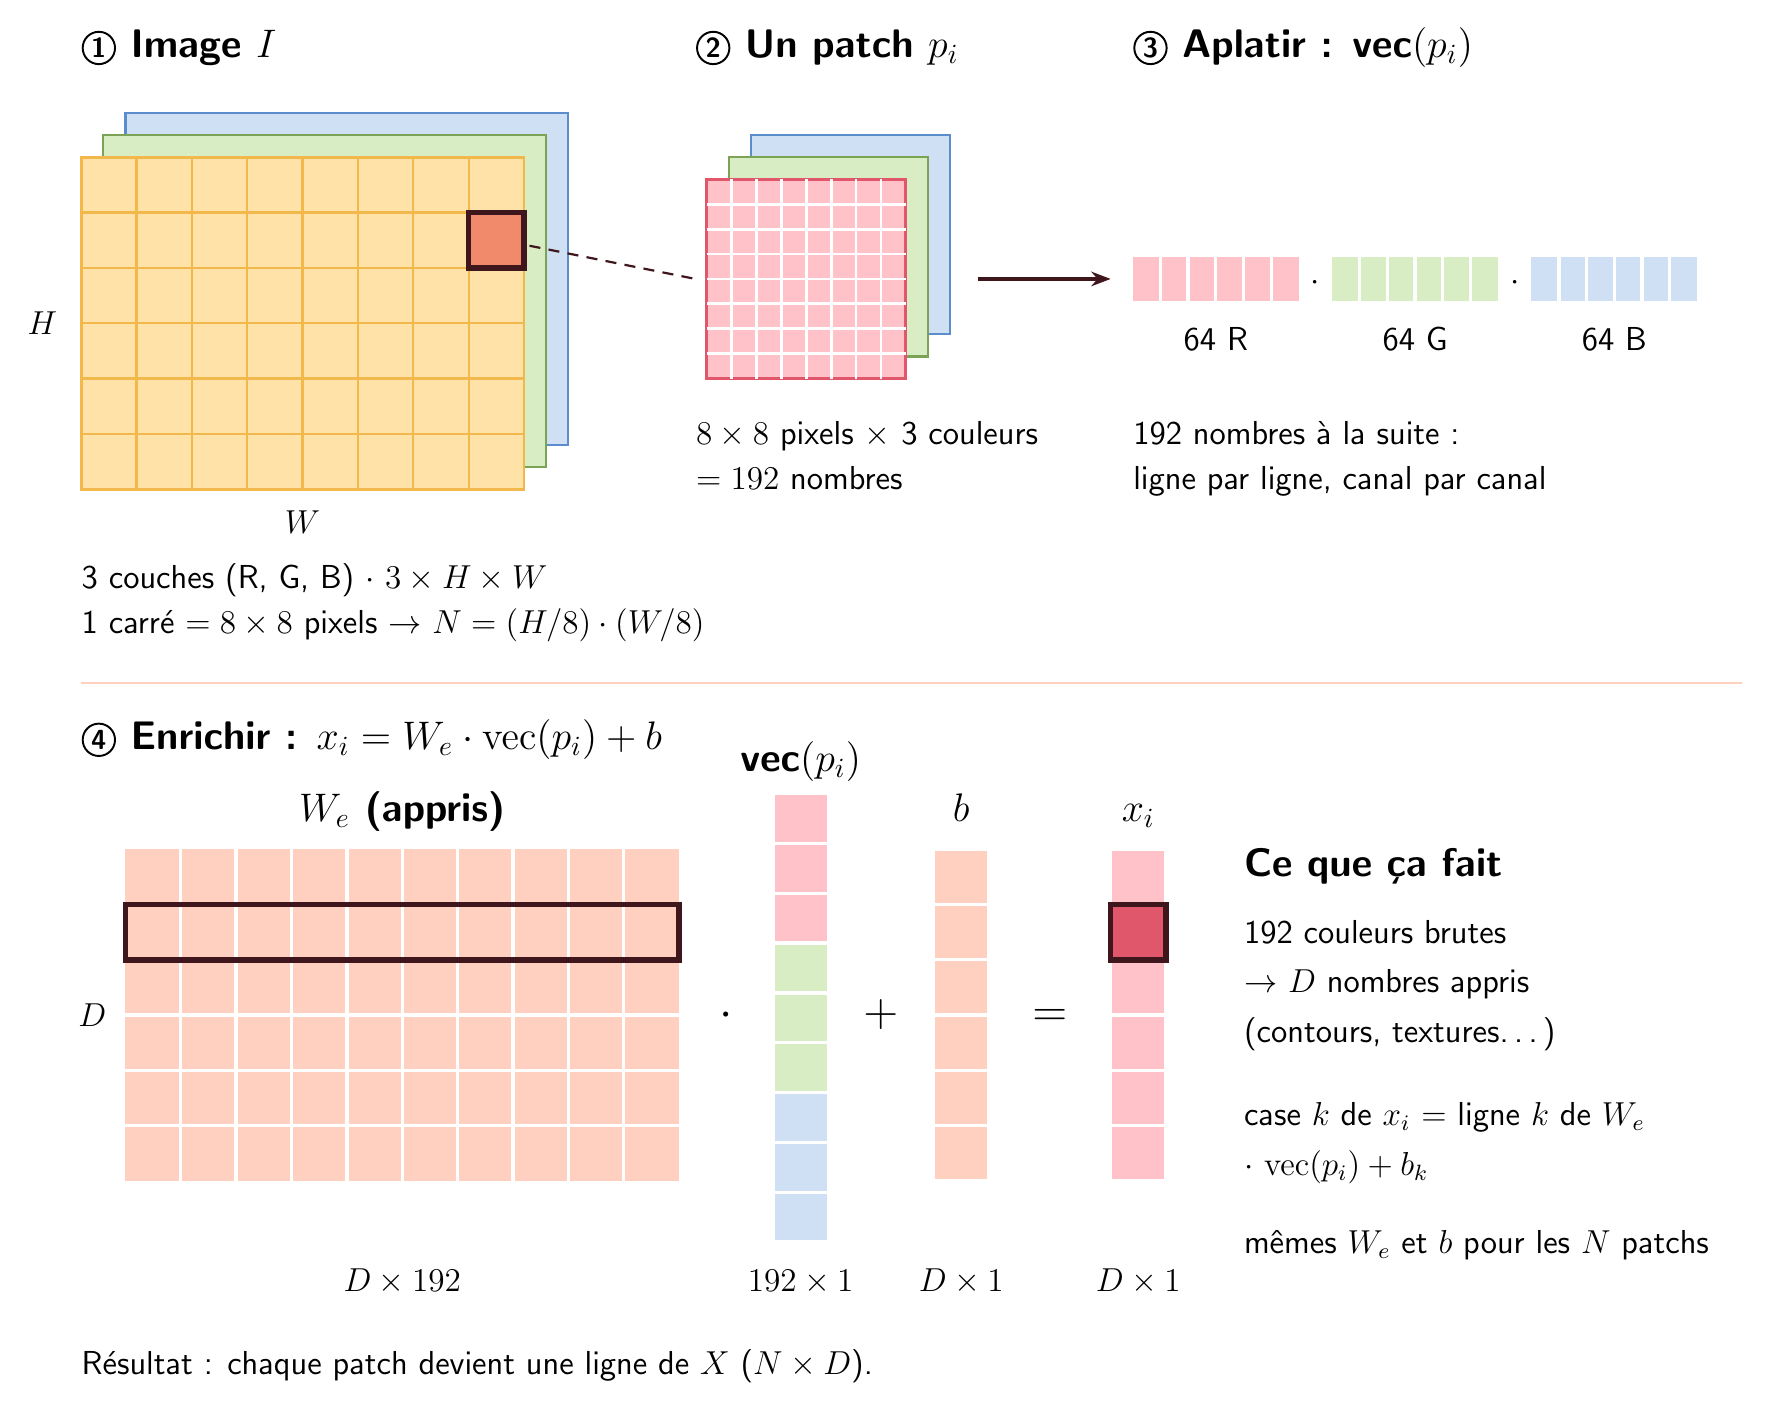
\begin{tikzpicture}[x=1pt, y=-1pt, line join=miter]

% ---------- Titres du haut ----------
\node[th, anchor=base west] at (40,24)  {\num{1} Image $I$};
\node[th, anchor=base west] at (262,24) {\num{2} Un patch $p_i$};
\node[th, anchor=base west] at (420,24) {\num{3} Aplatir : vec$(p_i)$};

% ---------- 1. Image I (3 couches) ----------
\filldraw[fill=bleu, draw=bleuB, line width=0.8pt] (56,44) rectangle (216,164);
\filldraw[fill=vert, draw=vertB, line width=0.8pt] (48,52) rectangle (208,172);
\filldraw[fill=jaune, draw=jauneB, line width=1pt] (40,60) rectangle (200,180);
\foreach \x in {60,80,...,180} \draw[jauneB, line width=0.8pt] (\x,60) -- (\x,180);
\foreach \y in {80,100,...,160} \draw[jauneB, line width=0.8pt] (40,\y) -- (200,\y);
\filldraw[fill=orangeF, draw=bordeaux, line width=2pt] (180,80) rectangle (200,100);
\node[ts, anchor=base] at (26,124) {$H$};
\node[ts, anchor=base] at (120,196) {$W$};
\node[ts, anchor=base west] at (40,216) {3 couches (R, G, B) $\cdot$ $3 \times H \times W$};
\node[ts, anchor=base west] at (40,232) {1 carré $= 8 \times 8$ pixels $\rightarrow$ $N = (H/8)\cdot(W/8)$};

% lien vers le zoom
\draw[bordeaux, line width=0.8pt, dash pattern=on 4pt off 3pt] (202,92) -- (262,104);

% ---------- 2. Patch p_i (8 x 8 x 3) ----------
\filldraw[fill=bleu, draw=bleuB, line width=0.8pt] (282,52) rectangle (354,124);
\filldraw[fill=vert, draw=vertB, line width=0.8pt] (274,60) rectangle (346,132);
\filldraw[fill=rose, draw=roseF, line width=1pt]   (266,68) rectangle (338,140);
\foreach \i in {1,...,7} {
  \draw[white, line width=1pt] (266+9*\i,68) -- (266+9*\i,140);
  \draw[white, line width=1pt] (266,68+9*\i) -- (338,68+9*\i);
}
\node[ts, anchor=base west] at (262,164) {$8 \times 8$ pixels $\times$ 3 couleurs};
\node[ts, anchor=base west] at (262,180) {$= 192$ nombres};

\draw[bordeaux, line width=1.5pt, -{Stealth[length=7pt]}] (364,104) -- (412,104);

% ---------- 3. Vecteur aplati (1 x 192) ----------
\fill[rose] (420,96) rectangle (480,112);
\fill[vert] (492,96) rectangle (552,112);
\fill[bleu] (564,96) rectangle (624,112);
\foreach \s in {420,492,564} {
  \foreach \k in {1,...,5} \draw[white, line width=1.2pt] (\s+10*\k,96) -- (\s+10*\k,112);
}
\node[ts, anchor=base] at (486,108) {$\cdot$};
\node[ts, anchor=base] at (558,108) {$\cdot$};
\node[ts, anchor=base] at (450,130) {64 R};
\node[ts, anchor=base] at (522,130) {64 G};
\node[ts, anchor=base] at (594,130) {64 B};
\node[ts, anchor=base west] at (420,164) {192 nombres à la suite :};
\node[ts, anchor=base west] at (420,180) {ligne par ligne, canal par canal};

% séparateur
\draw[orange, line width=1pt] (40,250) -- (640,250);

% ---------- 4. Enrichir ----------
\node[th, anchor=base west] at (40,274) {\num{4} Enrichir : $x_i = W_e \cdot \mathrm{vec}(p_i) + b$};

% W_e : D x 192
\node[th, anchor=base] at (156,300) {$W_e$ (appris)};
\fill[orange] (56,310) rectangle (256,430);
\foreach \x in {76,96,...,236} \draw[white, line width=1.2pt] (\x,310) -- (\x,430);
\foreach \y in {330,350,...,410} \draw[white, line width=1.2pt] (56,\y) -- (256,\y);
\draw[bordeaux, line width=2pt] (56,330) rectangle (256,350);
\node[ts, anchor=base] at (44,374) {$D$};

\node[op, anchor=base] at (273,374) {$\cdot$};

% vec(p_i) : 192 x 1
\node[th, anchor=base] at (300,282) {vec$(p_i)$};
\foreach \k/\c in {0/rose,1/rose,2/rose,3/vert,4/vert,5/vert,6/bleu,7/bleu,8/bleu}
  \filldraw[fill=\c, draw=white, line width=1.2pt] (290,290+18*\k) rectangle (310,308+18*\k);

\node[op, anchor=base] at (329,374) {$+$};

% b : D x 1
\node[th, anchor=base] at (358,300) {$b$};
\foreach \k in {0,...,5}
  \filldraw[fill=orange, draw=white, line width=1.2pt] (348,310+20*\k) rectangle (368,330+20*\k);

\node[op, anchor=base] at (390,374) {$=$};

% x_i : D x 1
\node[th, anchor=base] at (422,300) {$x_i$};
\foreach \k in {0,...,5}
  \filldraw[fill=rose, draw=white, line width=1.2pt] (412,310+20*\k) rectangle (432,330+20*\k);
\filldraw[fill=roseF, draw=bordeaux, line width=2pt] (412,330) rectangle (432,350);

% tailles
\node[ts, anchor=base] at (156,470) {$D \times 192$};
\node[ts, anchor=base] at (300,470) {$192 \times 1$};
\node[ts, anchor=base] at (358,470) {$D \times 1$};
\node[ts, anchor=base] at (422,470) {$D \times 1$};

% explication
\node[th, anchor=base west] at (460,320) {Ce que ça fait};
\node[ts, anchor=base west] at (460,344) {192 couleurs brutes};
\node[ts, anchor=base west] at (460,362) {$\rightarrow$ $D$ nombres appris};
\node[ts, anchor=base west] at (460,380) {(contours, textures\dots)};
\node[ts, anchor=base west] at (460,410) {case $k$ de $x_i$ = ligne $k$ de $W_e$};
\node[ts, anchor=base west] at (460,428) {$\cdot\ \mathrm{vec}(p_i) + b_k$};
\node[ts, anchor=base west] at (460,456) {mêmes $W_e$ et $b$ pour les $N$ patchs};

\node[ts, anchor=base west] at (40,500) {Résultat : chaque patch devient une ligne de $X$ ($N \times D$).};

\end{tikzpicture}
\end{document}
